\documentclass[a4paper,10pt]{article}
\usepackage[top=3cm, bottom=3cm, left=3cm, right=3cm]{geometry}
\usepackage[T1]{fontenc}
\usepackage[utf8]{inputenc}
\usepackage{lmodern}
\usepackage[francais]{babel}
\usepackage{graphicx}
\usepackage{caption}
\usepackage{subcaption}
\usepackage{eurosym}
\usepackage{hyperref}
\usepackage{csvsimple}
\usepackage{array}
\usepackage{longtable}
\usepackage{placeins}

\begin{document}

\begin{titlepage}
  \newcommand{\HRule}{\rule{\linewidth}{0.5mm}} % Defines a new command for the horizontal lines, change thickness here

  \center % Center everything on the page
   
  %----------------------------------------------------------------------------------------
  %	HEADING SECTIONS
  %----------------------------------------------------------------------------------------

  \textsc{\LARGE INSA de Lyon}\\[1.5cm] % Name of your university/college
  \textsc{\Large PLD-Agile}\\[0.5cm] % Major heading such as course name
  %\textsc{\large Compte rendue de TP}\\[0.5cm] % Minor heading such as course title

  %----------------------------------------------------------------------------------------
  %	TITLE SECTION
  %----------------------------------------------------------------------------------------

  \HRule \\[0.4cm]
  { \huge \bfseries Compte rendu de dernière itération}\\[0.4cm] % Title of your document
  \HRule \\[1.5cm]
   
  %----------------------------------------------------------------------------------------
  %	AUTHOR SECTION
  %----------------------------------------------------------------------------------------

  % If you don't want a supervisor, uncomment the two lines below and remove the section above
  \Large \emph{Auteurs:}\\[1cm]
  \begin{table}[h]
    \begin{center}
      \begin{tabular}{r l}
         Sebastien & \textsc{Di Giovanni} \\
         Hugo & \textsc{Moynac} \\
         Ruben & \textsc{Pericas Moya} \\
         François & \textsc{Robion} \\
         Charles & \textsc{Samborski} \\
         Nicolas & \textsc{Six} \\[3cm]
      \end{tabular}
    \end{center}
  \end{table}
  
  %----------------------------------------------------------------------------------------
  %	DATE SECTION
  %----------------------------------------------------------------------------------------

  {\large \today}\\[3cm] % Date, change the \today to a set date if you want to be precise

  %----------------------------------------------------------------------------------------
  %	LOGO SECTION
  %----------------------------------------------------------------------------------------

  %\includegraphics{Logo}\\[1cm] % Include a department/university logo - this will require the graphicx package
   
  %----------------------------------------------------------------------------------------

  \vfill % Fill the rest of the page with whitespace

\end{titlepage}
\tableofcontents
\pagebreak

\section{Glossaire}
  %generated using http://www.tablesgenerator.com/latex_tables by importing Google csv version
%des modification ont du être faitent à la main après...


\begin{longtable}{|p{0.2\linewidth}|p{0.2\linewidth}|p{0.5\linewidth}|}
\caption{Glossaire} \label{glossaire} \\

\hline \multicolumn{1}{|c|}{\textbf{Nom anglophone}} & \multicolumn{1}{c|}{\textbf{Nom francophone}} & \multicolumn{1}{c|}{\textbf{Définition}} \\ \hline 
\endfirsthead

\multicolumn{3}{c}%
{{\bfseries \tablename\ \thetable{} -- continued from previous page}} \\
\hline \multicolumn{1}{|c|}{\textbf{Nom anglophone}} & \multicolumn{1}{c|}{\textbf{Nom francophone}} & \multicolumn{1}{c|}{\textbf{Définition}} \\ \hline 
\endhead

\hline \multicolumn{3}{|r|}{{Continued on next page}} \\ \hline
\endfoot

\hline \hline
\endlastfoot


\hline
Delivery address                            & Adresse de livraison            & Identifie une intersection où une livraison doit être effectuée.                                                                                                                                                                                                                    \\ \hline
End (in street section, out street section)   & Arrivée (tronçon, intersection) & Intersection identifiant le point d'arrivée d'un tronçon.                                                                                                                                                                                                                           \\ \hline
Delivery constraint                         & Contrainte delivraison         & Plage horaire durant laquelle une livraison doit être effectué.                                                                                                                                                                                                                     \\ \hline
Delivery request                            & Demande de livraison            & Ensemble d'adresses de livraison, ainsi que l'entrepôt et lescontraintes de livraison associées.                                                                                                                                                                                    \\ \hline
Start(in street section, out street section) & Départ(tronçon, intersection)  & Intersection identifiant le point de départ d'un tronçon.                                                                                                                                                                                                                           \\ \hline
Delivery duration                           & Durée de livraison             & Temps pris par le livreur pour effectuer une livraison.                                                                                                                                                                                                                             \\ \hline
Warehouse                                   & Entrepôt                       & Point de départ et de fin d'une tournée.C'est une intersection particulière.                                                                                                                                                                                                        \\ \hline
Delivery graph                              & Graphe deslivraisons           & Graphe complet et orienté représentant l'ensemble des adresses de livraisons (noeuds), ainsi que les trajets pour aller d'une adresse de livraison à une autre (arc).                                                                                                                \\ \hline
Delivery Interval                           & Horairede passage              & Heure d'arrivé et heure de départ d'un livreur à une adresse livraison.                                                                                                                                                                                                             \\ \hline
Intersection                                & Intersection                   & Noeud du plan.                                                                                                                                                                                                                                                                      \\ \hline
Delivery                                    & Livraison                      & Action réalisée par le client qui consiste à s'arrêter un certain temps à une adresse de livraison.Peut être caractérisée par des contraintes de livraison.                                                                                                                         \\ \hline
Delivery man                                & Livreur                        & Personne effectuant les tournées.                                                                                                                                                                                                                                                   \\ \hline
City map                                    & Plan                           & Graphe orienté représentant le plan de la ville.                                                                                                                                                                                                                                    \\ \hline
Street                                      & Rue                            & Nom donné à un ensemble de tronçons partageant le même nom.                                                                                                                                                                                                                         \\ \hline
Street sectionlength                        & Taille de tronçon              & Longueur du tronçon (en mètres).                                                                                                                                                                                                                                                    \\ \hline
Wainting time                               & Temps d'attente                & Temps que le livreur attend à une adresse de livraison avant de pouvoir l'effectuer.                                                                                                                                                                                                \\ \hline
Street sectiontime                          & Temps de tronçon               & Temps mis par un livreur pour parcourir un tronçon.                                                                                                                                                                                                                                 \\ \hline
Planning                                    & Tournée                        & Ensemble ordonné d'adresses de livraison, de trajets entre ces adresses de livraison,et des horaires de passages à chacune des adresses de livraison.Le livreur commence sa tournée en partant de l'entrepôt donné,livre chaque adresse de livraison, et retourne au même entrepôt. \\ \hline
Way point                                   & Point de passage               & Défini indifférement un entrepôt ou une adresse de livraison.                                                                                                                                                                                                                       \\ \hline
Route                                       & Trajet                         & Suite consécutive de tronçons: le départ d'un tronçon doit être l'arrivée du tronçon précédent.Un trajet relie une adresse de livraison à une autre adresse de livraison (ou un entrepôt).                                                                                          \\ \hline
Street section                              & Tronçon                        & Arc du plan reliant deux intersections.Chaque tronçon possède un identifiant pour le différencier de la rue.Un tronçon est caractérisé par une intersection de départ et par une intersection d'arrivée.                                                                            \\ \hline
In streetsection                            & Tronçon entrant                & Tronçon arrivant sur une intersection.                                                                                                                                                                                                                                              \\ \hline
Out street section                          & Tronçon sortant                & Tronçon sortant d'une intersection.                                                                                                                                                                                                                                                 \\ \hline
\end{longtable}%


\FloatBarrier
\section{Modèle du domaine}
  \begin{figure}[h!]
    \begin{center}
      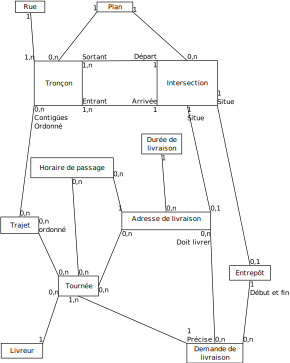
\includegraphics[width=0.7\linewidth]{images/Modele.png}
      \caption{Modèle du domaine}
      \label{fig:modele}
    \end{center}
  \end{figure}
  
\FloatBarrier
\section{Diagramme de cas d'utilisation}
  \begin{figure}[h!]
    \begin{center}
      \includegraphics[width=0.5\linewidth]{project/use-cases/UsesCases.png}
      \caption{Diagramme de cas d'utilisatione}
      \label{fig:useCase}
    \end{center}
  \end{figure}

\FloatBarrier
\section{Description textuelle des cas d’utilisation}
  \subsection{Ouvrir un plan}\hypertarget{ouvrir-un-plan}{}\label{ouvrir-un-plan}

\subsubsection{Préconditions}\hypertarget{prconditions}{}\label{prconditions}

\emph{(aucune)}

\subsubsection{Scénario}\hypertarget{scnario}{}\label{scnario}

\begin{enumerate}
\item L'utilisateur demande l'ouverture d'un plan.
\item Le système propose à l'utilisateur de choisir le fichier décrivant le plan.
\item Le système charge le plan et l'affiche
\end{enumerate}

\subsubsection{Alternatives}\hypertarget{alternatives}{}\label{alternatives}

\begin{itemize}
\item Le fichier est invalide, une erreur a lieu au chargement


\begin{itemize}
\item Annuler le chargement et afficher une erreur
\end{itemize}
\end{itemize}

  \subsection{Ouvrir une demande de livraison}\hypertarget{ouvrir-une-demande-de-livraison}{}\label{ouvrir-une-demande-de-livraison}

\subsubsection{Préconditions}\hypertarget{prconditions}{}\label{prconditions}

\begin{itemize}
\item Un plan est chargé
\end{itemize}

\subsubsection{Scenario}\hypertarget{scenario}{}\label{scenario}

\begin{enumerate}
\item L'utilisateur demande l'ouverture d'une demande de livraison.
\item Le système propose à l'utilisateur de choisir le fichier décrivant la demande de livraison.
\item Le système charge le plan et affiche ses données: entrepôt, adresses de livraison
et contraintes de livraison (horaires de passage).
\end{enumerate}

\subsubsection{Alternatives}\hypertarget{alternatives}{}\label{alternatives}

\begin{itemize}
\item Le fichier est invalide, une erreur a lieu au chargement


\begin{itemize}
\item Annuler le chargement et afficher une erreur
\end{itemize}
\end{itemize}

  \subsection{Calculer la tournée}\hypertarget{calculer-la-tourne}{}\label{calculer-la-tourne}

\subsubsection{Préconditions}\hypertarget{prconditions}{}\label{prconditions}

\begin{itemize}
\item Un plan est chargé
\item Une demande de livraison est chargée
\end{itemize}

\subsubsection{Scénario}\hypertarget{scnario}{}\label{scnario}

\begin{enumerate}
\item L'utilisateur demande de calculer la meilleure tournée possible pour la demande
de livraison chargée.
\item Le système essaie de calculer la meilleure tournée.
\item Le système affiche sa proposition pour la tournée.
\end{enumerate}

\subsubsection{Alternatives}\hypertarget{alternatives}{}\label{alternatives}

\begin{itemize}
\item Il n'existe aucune tournée possible.


\begin{itemize}
\item Afficher une erreur
\end{itemize}
\end{itemize}
 

\FloatBarrier
\section{Diagramme Etats-transitions}
  \begin{figure}[h!]
    \begin{center}
      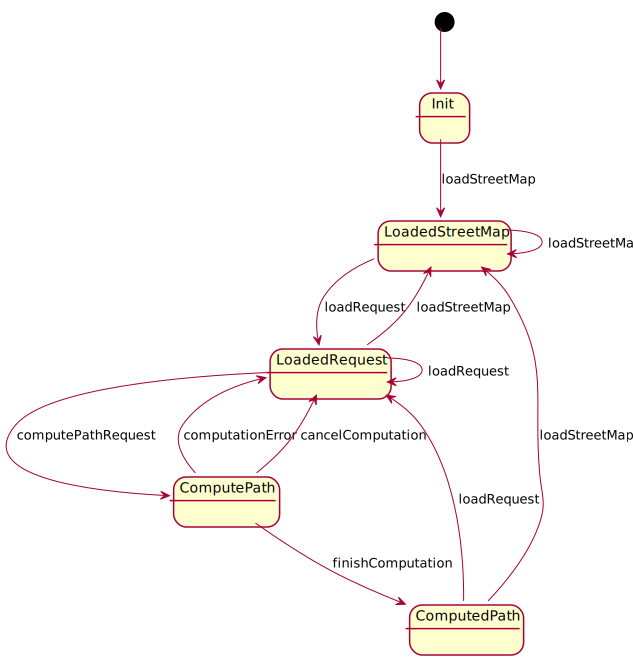
\includegraphics[width=0.8\linewidth]{uml/state-diagram-gui.png}
      \caption{Diagramme Etats-transitions}
      \label{fig:stateGui}
    \end{center}
  \end{figure}
  
  
\FloatBarrier
\section{Diagramme de packages et de classes}
  \begin{figure}[h!]
    \begin{center}
      \includegraphics[width=\linewidth]{uml/packages-summary.png}
      \caption{Résumé du diagramme de packages et de classes}
      \label{fig:packagesSummary}
    \end{center}
  \end{figure}
  \begin{figure}[h!]
    \begin{center}
      \includegraphics[width=.7\paperheight,angle=90]{uml/packages-overview.png}
      \caption{Diagramme de packages et de classes}
      \label{fig:packages}
    \end{center}
  \end{figure}
  \begin{figure}[h!]
    \begin{center}
      \includegraphics[width=0.8\linewidth]{{uml/package.model}.png}
      \caption{Diagramme de classes du modèle}
      \label{fig:packagesModel}
    \end{center}
  \end{figure}
  \begin{figure}[h!]
    \begin{center}
      \includegraphics[width=\linewidth]{{uml/package.services}.png}
      \caption{Diagramme de classes des services}
      \label{fig:packagesServices}
    \end{center}
  \end{figure}
  \begin{figure}[h!]
    \begin{center}
      \includegraphics[width=\linewidth]{{uml/package.components}.png}
      \caption{Diagramme de classes du controlleur}
      \label{fig:packagesServices}
    \end{center}
  \end{figure}

\FloatBarrier
\section{Diagramme de séquence du calcul de la tournée}
  \begin{figure}[h!]
    \begin{center}
      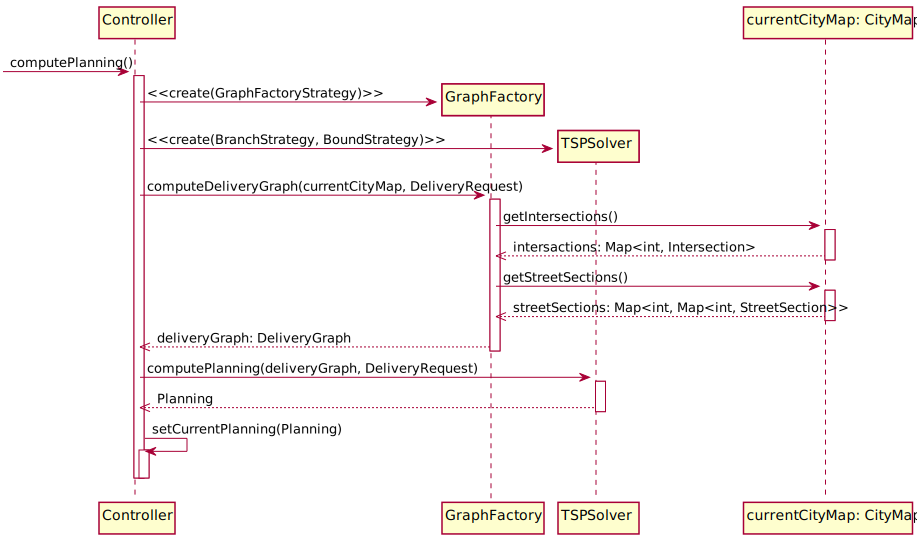
\includegraphics[width=\linewidth]{{uml/sequence-diagram-planning}.png}
      \caption{Diagramme de séquence du calcul de la tournée}
      \label{fig:sequencesTournee}
    \end{center}
  \end{figure}
  \begin{figure}[h!]
    \begin{center}
      \includegraphics[width=\linewidth]{{uml/sequence-diagram-tsp}.png}
      \caption{Diagramme de séquence de la résolution du TSP}
      \label{fig:sequencesTSP}
    \end{center}
  \end{figure}

\FloatBarrier
\section{Planning effectif de la première itération}
  \begin{longtable}{|p{0.4\linewidth}|l|l|c|c|}
\caption{Répartition des charges} \label{tab:charges} \\

\hline
\multicolumn{1}{|c|}{\textbf{Nom de tâche}} & \multicolumn{1}{p{0.1\linewidth}|}{\textbf{Acteur principal}} & \multicolumn{1}{p{0.1\linewidth}|}{\textbf{Acteur aide}} & \multicolumn{1}{p{0.1\linewidth}|}{\textbf{Temps estimé (heures)}} & \multicolumn{1}{p{0.1\linewidth}|}{\textbf{Temps passé (heures)} } \\ \hline
\endfirsthead 

\multicolumn{5}{c}%
{{\bfseries \tablename\ \thetable{} -- suite du tableau précédant}} \\
\hline
\multicolumn{1}{|c|}{\textbf{Nom de tâche}} & \multicolumn{1}{p{0.1\linewidth}|}{\textbf{Acteur principal}} & \multicolumn{1}{p{0.1\linewidth}|}{\textbf{Acteur aide}} & \multicolumn{1}{p{0.1\linewidth}|}{\textbf{Temps estimé (heures)}} & \multicolumn{1}{p{0.1\linewidth}|}{\textbf{Temps passé (heures)}}                   \\ \hline
\endhead

\hline \multicolumn{5}{|r|}{{Suite sur la page suivante}} \\ \hline
\endfoot

\hline \hline
\endlastfoot


Glossaire                            & Ruben            & François    & 2                    & 2                   \\ \hline
Diagramme entité association         & François         & Ruben       & 2                    & 1                   \\ \hline
Modèle du domaine                    & François         & Ruben       & 3                    & 3                   \\ \hline
Diagramme de cas d'utilisations      & Nicolas          & Hugo        & 1                    & 1                   \\ \hline
Diagramme de cas d'utilisations      & Charles          & Sébastien   & 1                    & 1                   \\ \hline
Tenue des charges                    & Ruben            &             & 0,5                  & 0,5                 \\ \hline
Diagramme Etats-transitions          & Nicolas          & Hugo        & 0,5                  & 0,5                 \\ \hline
Diagramme Etats-transitions          & Charles          & Sébastien   & 0,5                  & 3                   \\ \hline
Diagramme de packages et de classes  & Nicolas          & Hugo        & 3                    & 1,5                 \\ \hline
Diagramme de packages et de classes  & Charles          & Sébastien   & 4                    & 5                   \\ \hline
Package Model                        & François         & Ruben       & 4                    & 2                   \\ \hline
Package Services                     & Ruben            & Nicolas     & 2                    & 2                   \\ \hline
Diagramme séquence TSP               & Ruben            &             & 1                    & 1                   \\ \hline
Diagramme séquence TSP global        & Charles          & Ruben       & 1                    & 2                   \\ \hline
Codage du Parser CityMap             & François         &             & 3                    & 3                   \\ \hline
Maquette de l'IHM                    & Sébastien        & Hugo        & 4                    & 4                   \\ \hline
Diagramme de classe (pck controller) & Charles          & Sébastien   & 4                    & 4                   \\ \hline
Diagramme de classe (pck controller) & Hugo             &             & 4                    & 4                   \\ \hline
Manage backlog                       & Ruben            &             & 1                    & 1                   \\ \hline
Note: backlog                        & Ruben            &             & 0,5                  & 1                   \\ \hline
Codage du Parser DeliveryRequest     & François         &             & 1,5                  & 3                   \\ \hline
Dijkstra                             & Sébastien        & François    & 5                    & 7                   \\ \hline
Implémentation TSP                   & Ruben            & Nicolas     & 2                    & 3                   \\ \hline
Implémentation computeDeliveryGraph  & Sébastien        &             & 1                    & 1                   \\ \hline
Test de Parser.getDeliveryRequest    & François         &             & 2                    & 3                   \\ \hline
Suppressions des wrappers du modele  & François         &             & 0,5                  & 0,5                 \\ \hline
Test de computeDeliveryGraph         & Sébastien        &             & 2                    & 2                   \\ \hline
Amélioration de shortestPath         & Sébastien        &             & 1                    & 1                   \\ \hline
Debug du TSP                         & Ruben            & François    & 2                    & 3                   \\ \hline
Mises en forme LaTeX                 & Nicolas          &             & 4                    & 5                   \\ \hline
Mise en place de la GUI              & Charles          &             & 3                    & 5                   \\ \hline
Composant "Application"              & Charles          & Hugo        & 5                    & 8                   \\ \hline
Composant "MapCanvas"                & Hugo             & Charles     & 4                    & 7                   \\ \hline
Composant "MapScreen"                & Charles          &             & 0.5                  & 0.5                 \\ \hline
Composant "PlanningDetails"          & Charles          &             & 2                    & 2.5                 \\ \hline
Outils (Intégration, Documentation)  & Charles          & Ruben       & 10                   & 15                  \\ \hline
\end{longtable}


\end{document}
